\documentclass[a4paper,twoside,12pt]{book}
\usepackage[utf8]{inputenc}
\usepackage{natbib}
\usepackage{graphicx}
\usepackage[a4paper, left=37mm, right=27mm, top=39mm, bottom=39mm, headsep=12mm, footskip=15mm]{geometry}
\setlength{\headheight}{15pt}
\usepackage{fancyhdr}
\usepackage{fontenc}
\usepackage{float}
\usepackage{rotating}
\usepackage{hyperref}
\usepackage{afterpage}
\usepackage{mathtools}
\usepackage{amsmath}
\usepackage{tabu}
\usepackage{listings}
\usepackage{subcaption}
\usepackage{emptypage}
\usepackage{bookmark}
\usepackage{xfrac}
\usepackage{epsfig}

\pagestyle{fancy}
\renewcommand{\chaptermark}[1]{\markboth{#1}{}}
\renewcommand{\sectionmark}[1]{\markright{\thesection\ #1}}
\fancyhf{} \fancyhead[LE,RO]{\bfseries\thepage}
\fancyhead[LO]{\bfseries\rightmark}
\fancyhead[RE]{\bfseries\leftmark}
\renewcommand{\headrulewidth}{0.5pt}
\renewcommand{\footrulewidth}{0pt}
\fancypagestyle{plain}{
	\fancyhead{}
	\renewcommand{\headrulewidth}{0pt}}

%%%%%%%%%% General thesis informations go here! (TITLE, AUTHOR-NAME, KEYWORD-1, KEYWORD-2,...
\hypersetup{
    pdfauthor  = {AUTHOR-NAME},    		    % author
    pdftitle   = {TITLE},    				% title
 	pdfsubject = {Master's Degree Thesis},  % subject of the document
 	pdfkeywords= {KEYWORD-1, KEYWORD-2}      % list of keywords
}

%%%%%%%%%%%%%%%%%%%%%%%%%%%%%% BEGIN OF THE DOCUMENT
\begin{document}

\pagestyle{fancy}
\renewcommand{\chaptermark}[1]{\markboth{#1}{}}
\renewcommand{\sectionmark}[1]{\markright{\thesection\ #1}}
\fancyhf{} \fancyhead[LE,RO]{\bfseries\thepage}
\fancyhead[LO]{\bfseries\rightmark}
\fancyhead[RE]{\bfseries\leftmark}
\renewcommand{\headrulewidth}{0.5pt}
\renewcommand{\footrulewidth}{0pt}
\fancypagestyle{plain}{
	\fancyhead{}
	\renewcommand{\headrulewidth}{0pt}}

%%%%%%%%%%%%%%%%%%%%%%%%%%%%%% Title page	
\newgeometry{margin=3cm}
\begin{titlepage}

%%%%%%%%%% Department informations go here!
\begin{center}
\Large{\textbf{\textsc{Politecnico di Milano}}}\\
\Large{\textbf{School of Industrial and Information Engineering}}\\
\large{\textbf{Computer Science and Engineering Course}}\\
\par
\end{center}

\vspace{0.2cm}

\begin{center}
\begin{figure}[h]
\centering{}
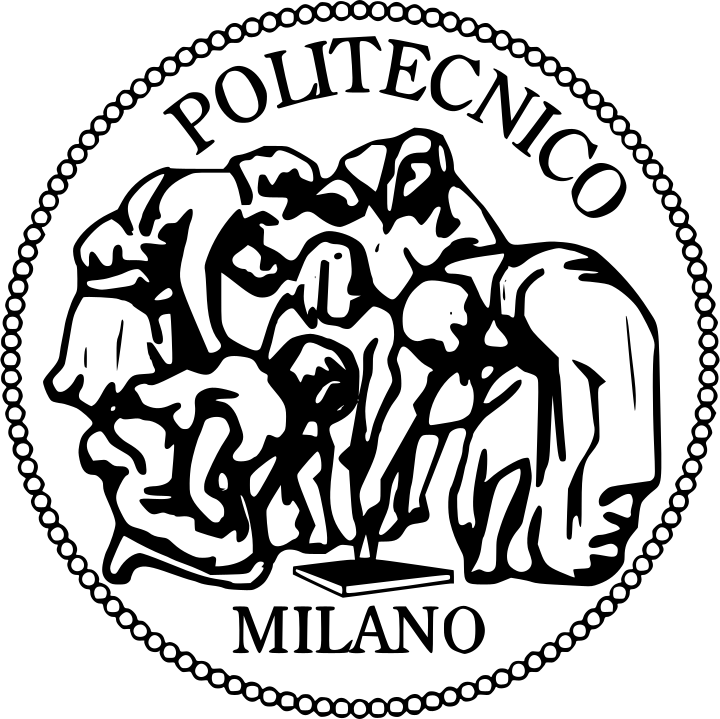
\includegraphics[width=0.3\textwidth]{title-page/logo-polimi}
\end{figure}
\par
\end{center}

%%%%%%%%%% Thesis title goes here!
\begin{center}
\LARGE{\textbf{Consensus based control for a} \\\textbf{Unmanned Aerial Vehicle formation}}
\vspace{1.0cm}
\par
\end{center}

%%%%%%%%%% Advisor and co-advisor names go here!
\begin{flushleft}
\begin{tabular}{ll}
\textbf{Advisor:}      & \textbf{Prof. Marco LOVERA}\tabularnewline
\textbf{Co-Advisors:}  & \textbf{Eng. Pietro PANIZZA}\tabularnewline
                       & \textbf{Eng. Mattia GIURATO}\tabularnewline
\end{tabular}\vspace{0.3cm}
\par
\end{flushleft}

%%%%%%%%%% Student name goes here!
\begin{flushright}
\begin{tabular}{ll}
\textbf{Thesis by:} & \tabularnewline
\textbf{Alex DELBONO} & \textbf{Matr. 850114}\tabularnewline
\end{tabular}\vspace{1cm}
\par
\end{flushright}

\begin{center}
{\large{}\textbf{Academic Year 2016\textendash 2017}}
\par
\end{center}{\large \par}

\end{titlepage}

\restoregeometry

\cleardoublepage{}

%%%%%%%%%%%%%%%%%%%%%%%%%%%%%% Dedication
\begin{flushright}
\emph{A Pietro, una persona vera ed altruista come poche\ldots{}
}
\cleardoublepage{}
\par
\end{flushright}

%%%%%%%%%%%%%%%%%%%%%%%%%%%%%% Acnowledgment
\chapter*{Acknowledgments}
\addcontentsline{toc}{chapter}{Acknowledgments}
%«È di cattivo gusto ringraziare il relatore. Se vi ha aiutato ha fatto solo il suo dovere» Uberto Eco, Come si fa una tesi di laurea


%%%%%%%%%%%%%%%%%%%%%%%%%%%%%% Abstract
\chapter*{Abstract}
\addcontentsline{toc}{chapter}{Abstract}
%The abstract must contain 3 main logic blocks which will be discussed in the introduction.

%Field of work
%The first block must contain a sentence which describes the field of work, and eventually another sentence which focuses the specific objective of the work in details.

%Purpose of the thesis
%The second block must start with the words «The purpose of the thesis is …».

%Short recap
%The last block must summarize the conducted activities and the obtained results (evaluating them eventually).

This thesis is about the synchronized flight of a formation of multirotors which execute a mission.
The mission is characterized by a trajectory for each drone which composes the formation.
The formation must be able to deal with unforeseen events, which can compromise
the outcome of the mission. In order to do that, the drones must exchange information
with each others and a support network is therefore needed.

The purpose of this thesis is to present the algorithm for synchronized formation flight
called consensus algorithm and implement it in a simulated environment
and in a real system with heterogeneous drones. We want to verify that the theoretical
results can be applied in a real distributed system, with not ideal network performances.

In the first part, we explain the algorithm used during the experimental work,
while in the following chapter the software and hardware used are presented.
In the last chapters, we show in detail the structure of the software and the experiment conducted.
In particular, many simulations will be presented to confirm the quality of the
consensus algorithm. Finally, a comparison between the simulated results and the ones
obtained in the real environment is proposed.


%%%%%%%%%%%%%%%%%%%%%%%%%%%%%% Sommario
\chapter*{Sommario}
\addcontentsline{toc}{chapter}{Sommario}
%Il testo delle tesi redatte in lingua straniera dovrà essere introdotto da un ampio estratto in lingua italiana, che andrà collocato dopo l’abstract.

La tesi tratta di volo sincronizzato di una formazione di multirotori che eseguono una missione,
caratterizzata da una traiettoria per ogni drone che compone la formazione.
La formazione deve essere in grado di reagire a eventi inaspettati, che possono
compromettere l'esito della missione stessa.
Per raggiungere tale scopo, i droni devono scambiare informazioni, attraverso
una rete di supporto.

L'obbiettivo della tesi è di presentare l'algoritmo utilizzato per il volo sincronizzato,
chiamato algoritmo di consenso e implementarlo sia in un ambiente simulato,
che in un sistema reale, composto da macchine eterogenee. Si vuole verificare che
i risultati teorici possano essere applicati in un sistema reale distribuito, dotato di
una rete di comunicazione dalle prestazioni non ideali.

Nella prima parte della tesi, verrà esposto l'algoritmo usato durante il lavoro sperimentale,
mentre nel capitolo seguente saranno presentati l'hardware e il software.
Negli ultimi capitoli saranno evidenziati nel dettaglio la struttura del software
e gli esperimenti condotti.
In particolare, saranno mostrate alcune simulazioni, in modo da confermare la bontà
dell'algoritmo di consenso.
Infine, nell'ultimo capitolo, sarà proposta una comparazione tra i risultati
delle simulazioni e quelli ottenuti mediante l'implementazione in un sistema reale.

\tableofcontents 

%%%%%%%%%%%%%%%%%%%%%%%%%%%%%% List of figures
\listoffigures
\addcontentsline{toc}{chapter}{List of figures}
\cleardoublepage{}

%%%%%%%%%%%%%%%%%%%%%%%%%%%%%% List of tables
\listoftables
\addcontentsline{toc}{chapter}{List of tables}
\cleardoublepage{}

%%%%%%%%%%%%%%%%%%%%%%%%%%%%%% Introduction
\chapter*{Introduction\label{chap:introduction}}
\addcontentsline{toc}{chapter}{Introduction}
\markboth{Introduction}{Introduction}
%The introduction must be atomic, it does not have to include subsections nor paragraphs.

%The title, the abstract and the introduction must appear as chinese boxes: if read in this order, they must progressively show the informations about the topic in order to catch the attention of the reader.

%The introduction must be divided in three main logic blocks as well:
%General overview
%A brief description of the work
%Structure of the thesis

These years are characterized by the development of the robotics.
The growing applications of mobile robots and drones in many fields
has brought important increasing in the number of robotic vehicles.
Many commercial solutions are available, but in many cases they offer
a product which needs an expert pilot. For this reason and due to the high prices,
the diffusion of mobile robots is limited. In the latest years, these problems were
mitigated and we now see lower prices and easier to use products. This will bring a
growing non professional diffusion of robotic vehicles which, hopefully, will populate
our houses and help us in our life.
The most important application of UAVs are the ones related to exploration and data
collection. Indeed, drones are fundamental in inspection of unknown areas, such as
forests or unreachable terrains.
Also the monitoring of industrial artifacts constitutes a valuable application of UVAs.
For instance, solar panels, wind turbines, high-voltage cables or tubes can be
supervised using aerial vehicles.
The multimedia production is the field in which the drones are most present. Indeed,
most of the machines are equipped with high-definition cameras in order to provide
professional videos.

The power consumptions of the machines are significantly reduced in the last years
and we are now able to build smaller and lighter vehicles.
In particular, in the aerial field, there are commercial products which weight
about 200g with a flight time of 20 minutes.
These improvements allow us to develop more advanced features, such as
trajectory planning, obstacles avoidance, formation flight.
The development of autonomous UAVs is fundamental in application such as humanitarian
response around the world. When a natural calamity happens, the UAVs can play a
crucial role, delivering essential goods or finding missing people. Moreover, the
operations can be done without risking the safety or life of the rescuers, because
they can act remotely or plan an autonomous mission.

The trajectory planning is essential for the development of autonomous vehicles,
because the generation of a feasible trajectory for a mission is a requirement,
otherwise no mission can be done.
The trajectory generation is an hard problem, because of its computational complexity.
Indeed, many suboptimal algorithm have been developed in order to reduce the
complexity.
There are different classes of planning algorithm and they can be summarized as follows:
\begin{itemize}
  \item Artificial Potential Field: these algorithms assigns a value of the potential
  for every point in the map. The goal has the lowest (highest) value and the obstacles
  have high (low) values. Then, the robot tries to descend (climb) the potential,
  in order to reach the goal.

  \item Sampling Based Planning: random samples are used to find a path from the
  starting point to the goal. Advanced random samples techniques can be used in order
  to reduce the complexity of the algorithm.

  \item Grid Based Planning: these kind of algorithm overlay a grid on the map, so
  every configuration corresponds with a grid pixel.
  The robot can move from one grid pixel to any adjacent grid pixels as long
  as that grid pixel does not contain an obstacle.

  \item Reward-Based Planning: the robot can apply different actions in every state
  of the world. The outcome of an action can be not deterministic and after every
  action, the robot gains a reward. The objective of the robot is to maximize the
  sum of the rewards.
\end{itemize}

Another important aspect is the obstacle avoidance. The trajectory usually is planned
offline, when the mission is not started yet. So, the trajectory does not take into
account the fact that an unplanned obstacle might interfere with the mission. In this
case another algorithm is implemented in order to run online. This kind of algorithms
are called obstacle avoidance algorithms and they replan locally the trajectory, in
order to get rid of unforeseen events. These algorithms need the drone to be equipped
with proximity sensors, which provide information about the surrounding environment.
Different methodologies have been developed for obstacles avoidance. The main ones are
summarized below without details.

\begin{itemize}
  \item Artificial Potential Field: as before, the idea of this approach is that
  obstacles exert a virtual repulsive force, given by the potential field, to push
  away the robot from them and the goal position generates a virtual attractive
  force to guide the robot to it.

  \item Virtual Force Field method (VFF): is the combination of the Artificial Potential
  Field with the concept of Probabilistic Occupancy Grid maps.

  \item Fuzzy Controller for Obstacle Avoidance: as the name says, a fuzzy controller
  is used to derives the variable for the vehicle’s orientation and acceleration,
  depending on the current perception of the robot’s sensors

  \item Vector Field Histogram method (VFH): improved version of the VFF method.

  \item VFH+, VFH$^*$ method: improved versions of the VFH method, but more computational costly.
  The most recent one is the VFH method, which uses an A$^*$ search.

  \item Traversability Field Histogram (TFH): The local path planner bases on
  the VFH concept but is extended by the information provided within the Traversability Map.

  \item Dynamic Window Approach: the algorithm takes into account the dynamic and kinematic constraints
  of the robot and it is similar to the VFH+ algorithm. The method is called
  dynamic window approach and considers only admissible velocities which can be
  reached within the next time interval and which allow the robot to stop safely.

  \item Curvature Velocity Space method: This method chooses a point in the linear-angular
  velocity space which satisfies some constraints and maximizes an objective function.
  This objective function tries to move the robot close to the commanded direction at
  the highest feasible speed, while travelling the trajectory with the largest clearance from obstacles.

  \item Beam Curvature method: improvement for the curvature velocity space method.

  \item Nearness diagram Navigation: it is similar to the VFH method, but uses
  a polar histogram to derive actions to be taken for the robot.
\end{itemize}

When multiple machines have to fly in a formation, a synchronization mechanism is
needed. Indeed, if one of the drones has to deviate from the planned trajectory
(for instance, because of an unplanned obstacle), the formation must be preserved.
To reach the synchronization, the vehicles must communicate with each others and
exchange information.
Notions from graph theory are needed to analyze the behaviour of the system
and demonstrate the convergence properties.

This work is focused on the presentation of a distributed synchronization algorithm,
which we call "Consensus Algorithm". Every drones must exchange its mission progression
with its neighbors and must adjust its mission progression based on the information
received from the other vehicles.
The algorithm is a distributed algorithm and it is executed on every vehicles.


In the first chapter, we will show the theoretical aspects of the of the "Consensus Algorithm".
Then, we will provide a general overview of the hardware and software used to deploy the algorithm.
In the third chapter we will show the software implementation of the main part of the
system, providing classes and snippets of code.
At the end, we will explain in the fourth and fifth chapters the simulated and experimental results of
our work. We will apply the algorithm to a real system and we will present our results and its
performances.


%%%%%%%%%%%%%%%%%%%%%%%%%%%%%% Chapter 1
\chapter{First chapter\label{chap:first-chapter}}
\section{Lorem ipsum}
Lorem ipsum dolor sit amet, consectetur adipiscing elit. Quisque lectus
mi, aliquet ac lectus at, luctus ornare enim. Donec eleifend ornare
ante. Curabitur non adipiscing risus. Vivamus congue sem non magna
tristique, ut pellentesque diam ornare. Donec eget arcu congue, vulputate
nisl et, aliquam tellus. Morbi tincidunt odio quis mi hendrerit aliquet
sit amet sit amet lorem. Donec fringilla nec lectus nec lacinia. Aliquam
eu nunc euismod, tempus neque in, consequat velit. Duis arcu quam,
convallis quis ultricies vitae, semper in est. Aliquam congue sagittis
tortor, eget blandit lorem ullamcorper id. Maecenas venenatis nec
neque in consectetur. Nulla nisl turpis, elementum a enim interdum,
tincidunt vehicula tortor. Praesent pulvinar mi sit amet condimentum
placerat. Curabitur mollis libero non auctor condimentum. Suspendisse
ante lectus, sodales vel mauris vel, pharetra laoreet eros.

Nam lacinia nunc lorem, adipiscing ornare purus semper sit amet. Morbi
elementum augue vitae purus vehicula, ac varius leo sagittis. Vestibulum
eu orci in ipsum suscipit posuere. Nulla quis erat rhoncus risus rutrum
venenatis vel at lectus. Vivamus pharetra tempor rhoncus. Proin vitae
turpis vitae lacus ultrices lacinia eu ac nunc. Morbi id metus purus.
Pellentesque facilisis at arcu ut adipiscing. Etiam eu nisi hendrerit,
congue orci non, vehicula orci. Interdum et malesuada fames ac ante
ipsum primis in faucibus. Aenean porttitor eu velit sed pulvinar.
Class aptent taciti sociosqu ad litora torquent per conubia nostra,
per inceptos himenaeos. Maecenas ut pretium nisi, nec aliquam massa.
Maecenas vitae rhoncus lacus, non tempus turpis.

Nam luctus in nisi dignissim congue. Nullam dapibus dui sed ligula
euismod congue. Nulla vestibulum, justo a feugiat porttitor, massa
nunc molestie lectus, ultrices tempus turpis massa posuere augue.
Phasellus pulvinar vulputate ipsum, et eleifend sapien mollis vel.
Sed vitae eros id sapien dictum ultricies. Aliquam ultricies nisl
et bibendum imperdiet. Cras a sem eros. Quisque ut mauris a libero
hendrerit tincidunt ac ac mi. Mauris feugiat est sem, eu malesuada
ipsum faucibus id. Duis at ante et justo ullamcorper hendrerit sed
ut turpis. Donec eu dolor ac enim venenatis placerat venenatis vitae
velit. Curabitur lacus nisi, molestie id ligula vel, congue porta
felis. Nam eu aliquam justo. Mauris sapien nulla, accumsan id eros
a, porttitor interdum nunc.

Vestibulum aliquam et mauris imperdiet consectetur. Pellentesque convallis
metus dignissim neque tincidunt, egestas commodo odio rhoncus. Integer
purus leo, posuere non leo eget, aliquet condimentum neque. Quisque
non hendrerit quam. Phasellus sit amet neque quam. Suspendisse at
sollicitudin ante. Mauris fermentum turpis eget sem cursus tempor.
Fusce ac rutrum libero, sed adipiscing diam.

Praesent quis ultricies diam, in hendrerit nibh. Praesent diam dolor,
bibendum sit amet pharetra a, viverra vel tortor. Mauris id eleifend
diam. Maecenas tristique est massa, et lacinia ante tristique nec.
Praesent sapien odio, iaculis sollicitudin tristique vitae, mattis
non lacus. Ut vehicula enim pellentesque, mollis ante vitae, mollis
mauris. Aenean imperdiet tellus lorem, eget malesuada ante rhoncus
id. Pellentesque dignissim nisl id pretium condimentum. Sed congue
commodo massa in rhoncus. Phasellus elementum sollicitudin erat id
rhoncus. Fusce sem nunc, semper at tempor sit amet, congue nec orci.
Vivamus a egestas dui, vel viverra eros. Sed sit amet eros sit amet
nisi gravida ullamcorper. Nam rutrum in mi sit amet vulputate. Aenean
pellentesque velit eu nisi eleifend faucibus sit amet vel dui. Pellentesque
sapien est, auctor at fringilla vel, vehicula ut urna \cite{Dijkstra68Letters}.

%%%%%%%%%%%%%%%%%%%%%%%%%%%%%% Chapter 2
\chapter{Second chapter\label{chap:second-chapter}}
\input{chapters/chapter-2/chapter-2.tex}

%%%%%%%%%%%%%%%%%%%%%%%%%%%%%% Chapter 3
\chapter{Third chapter\label{chap:third-chapter}}
\input{chapters/chapter-3/chapter-3.tex}

%%%%%%%%%%%%%%%%%%%%%%%%%%%%%% Chapter 4
\chapter{Fourth chapter\label{chap:fourth-chapter}}
\input{chapters/chapter-4/chapter-4.tex}

%%%%%%%%%%%%%%%%%%%%%%%%%%%%%% Chapter 5
\chapter{Fifth chapter\label{chap:fifth-chapter}}



%%%%%%%%%%%%%%%%%%%%%%%%%%%%%% Chapter 6
\chapter{Sixth chapter\label{chap:sixth-chapter}}



%%%%%%%%%%%%%%%%%%%%%%%%%%%%%% Chapter 7
\chapter{Seventh chapter\label{chap:seventh-chapter}}



%%%%%%%%%%%%%%%%%%%%%%%%%%%%%% Chapter 8
\chapter{Eighth chapter\label{chap:eighth-chapter}}



%%%%%%%%%%%%%%%%%%%%%%%%%%%%%% Chapter 9
\chapter{Ninth chapter\label{chap:ninth-chapter}}



%%%%%%%%%%%%%%%%%%%%%%%%%%%%%% Conclusion
\chapter*{Conclusions}
\addcontentsline{toc}{chapter}{Conclusions}
\markboth{Conclusions}{Conclusions}
%The conclusions must recall the field of work, the purpose of the thesis, what has been done and an evaluation of the obtained results.
%Furthermore, the conclusion must also emphasize the future prospects and must show how to move forward in the study area.

The results obtained in our experiments can be applied in many fields in which
a formation of UAVs has to operate.
In this thesis, we have shown how the consensus algorithm is deployed on a real
system and which performances can be achieved.

The implementation allows us to plan and fulfill a cooperative
mission in which the synchronization is one of the most important aspects.
The system is robust to network delays and loss of packets and to unexpected failures
of the vehicles involved.
Moreover, the formation, if equipped with an obstacle avoidance algorithm,
overcomes the presence of unexpected obstacles during the execution of the mission.

Further studies can be carried on in order to integrate recovery procedures in case
of network failures or the loss of a machine.
It is possible to develop obstacle avoidance algorithms or any kind of online procedures
acting directly on the free parameters of the algorithm presented.
In particular, it is possible to change the values of $\ddot{\gamma_d}$ and $\dot{\gamma_d}$,
in order to modify the velocity of the execution of the mission. These two values
can be also used to build more complex functionalities on top of the consensus algorithm.


%%%%%%%%%%%%%%%%%%%%%%%%%%%%%% Bibliography
\bibliographystyle{plain}
\bibliography{bibliography}

%%%%%%%%%%%%%%%%%%%%%%%%%%%%%% Appendix A
\appendix
\chapter{First appendix\label{app:first-appendix}}



%%%%%%%%%%%%%%%%%%%%%%%%%%%%%% Appendix B
\chapter{Second appendix\label{app:second-appendix}}



%%%%%%%%%%%%%%%%%%%%%%%%%%%%%% Appendix  C
\chapter{Third appendix\label{app:third-appendix}}


\cleardoublepage{}

%%%%%%%%%%%%%%%%%%%%%%%%%%%%%% END OF THE DOCUMENT
\end{document}